\subsection{Team Management}
  \subsubsection{Software Design Methodology}
    Throughout our project we followed an Agile software design approach in order to increase group productivity and accelerate code development. We felt that this enabled rapid response to alterations in project requirements and also provided a key factor in ensuring the project progressed according to plan.

    As a group we set milestones to monitor group progress and we ensured that the milestones where met consistently. This was essential in ensuring that the project was delivered on time considering the size and short timescale of the project. Milestones where set consisting of the the requirements outlined in weekly supervisor group meetings. Our Agile approach stimulated group responsiveness to changes in requirements (and new requirements defined in such milestones) by allocating specific tasks for each group member. 

    At a more detailed level within each milestone, we set iterations during frequent group stand up meetings in order to clarify individual member roles and tasks. In order to delegate tasks between the members of the group we divided up the group into Front-end, Back-end and Testing specialist units. Tasks outlined in each iteration would be divided accordingly to the corresponding units and then further assigned to individual group members. We used Trello in the initial stages of the project in order to allocate and divide tasks within iterations to group members, this provided an invaluable project management tool to establish group collaboration and roles. Towards the later stage of the project as group collaboration developed further, and the volume of new tasks decreased, we utelised GitHub\cite{github} issues to outline development issues that needed to be resolved, assigning issues to the specialised group member as they arose from testing and requirement changes.

    We felt that github issues were better than a white board of post it issues in a static location because not only does github allow you could access them at anytime, anywhere, you can assign different brightly coloured labels to the issues, assign them to a person to complete, comment on the issues and actually see the commits that fixed/broke these issues. 

    \begin{center}
    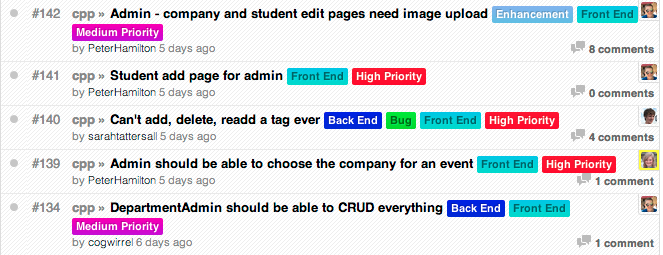
\includegraphics[scale=0.3]{images/project_management/team_management/github_issues}

    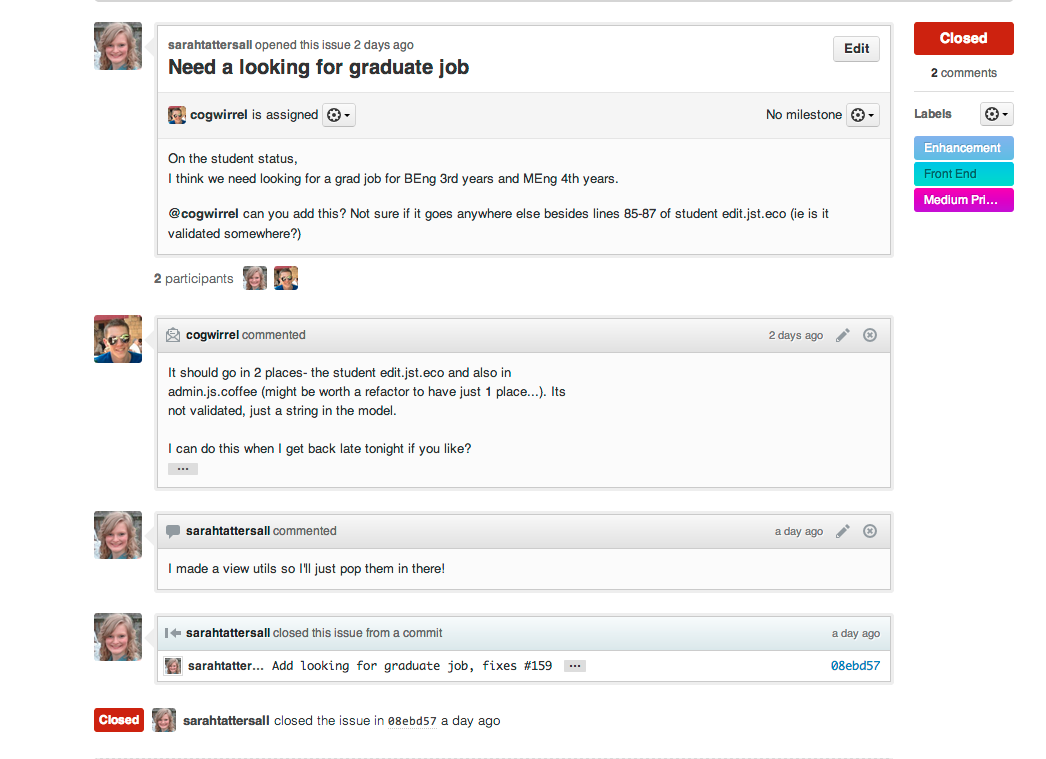
\includegraphics[scale=0.3]{images/project_management/team_management/graduate_issue}
    \end{center}


  \subsubsection{Team Collaboration}
    Through the use of frequent stand up meetings combined with daily group programming sessions and online communication, we established a very effective group development environment. We often developed alongside at least one other member of the group, using a specific area in the labs to work on the project which became a hub for development. We employed a collaborative approach to development, continuously communicating with each other for advice or alternative implementations, this enhanced development as each member had specific roles however as a group we maintained an overall understanding of the system and progress and so could collaboratively help each other.

    Our collaborative group environment was supported by the use of multiple collaboration tools, we used a GitHub repository and GIT\cite{git} as a version control system which allowed group members to work on development of their specific areas of functionality and merge the changed made by different members to the same files. Changes can also be reverted to previous versions at any time. GIT also enabled us to create separate braches for large sections of development that can be later integrated or dropped, for example we created a branch when we started to use Backbone in the early stages of the project. Overall GIT enabled us to develop simultaneously as a group to develop individually but merge changes frequently, iteratively adding assigned functionality. We extensively utelised GitHub issues to assign one or more members to tasks. Tags and comments can be associated with GitHub issues which can also be closed via GIT commits. GitHub issues are notified via email to all following members of the issue to update the status of the issue. These features all provided valuable in efficient code collaboration (... pull req ...). We also setup a Facebook group including all members to instantly message the entire group, this sustained the collaborative group environment and enabled the group to remain in instant contact when working remotely. 

    We used a continuous integration tracker called CircleCI to continuously report on the state of the project, alerting us if the build broke. As we developed we always aimed to maintain the build and found that this encouraged the flow of development as additions where integrated faster into an efficient and stable system advancement.
    We felt that writing weekly reports for the Software Engineering course enabled us to reflect on the group interaction and continuously reminded us to track our progress and apply an Agile development approach.   